% % % % % % % % % % % % % % % % % % % %
% Presentation Preamble
% % % % % % % % % % % % % % % % % % % %

\documentclass[mathserif]{beamer}

\mode<presentation>
{
	\usecolortheme{tum}
	\useoutertheme{tum}
	\useinnertheme{rectangles}

	\setbeamerfont{author}{size=\footnotesize}
	\setbeamerfont{date}{size=\scriptsize}
	\setbeamerfont{frametitle}{family=\rmfamily}

	\setbeamertemplate{title page}
	{
		\vbox{}
		\vfill
		\begin{flushleft}
			\begin{beamercolorbox}[sep=8pt,left]{title}
				\usebeamerfont{title}\inserttitle\par%
				\ifx\insertsubtitle\@empty%
				\else%
					\vskip0.25em%
					{\usebeamerfont{subtitle}\usebeamercolor[fg]{subtitle}\insertsubtitle\par}%
				\fi%
			\end{beamercolorbox}%
			\vskip1em\par
			\begin{beamercolorbox}[sep=8pt,left]{author}
			\usebeamerfont{author}\insertauthor
			\end{beamercolorbox}
			\begin{beamercolorbox}[sep=8pt,left]{institute}
			\usebeamerfont{institute}\insertinstitute
			\end{beamercolorbox}
			\begin{beamercolorbox}[sep=8pt,left]{date}
			\usebeamerfont{date}\insertdate
			\end{beamercolorbox}\vskip0.5em
			{\usebeamercolor[fg]{titlegraphic}\inserttitlegraphic\par}
		\end{flushleft}
		\vfill
	}

  \setbeamertemplate{footline}{}
	\setbeamertemplate{page number in head/foot}[framenumber]
	% Outer raisebox adds space to logo
	\setbeamertemplate{navigation symbols}{\raisebox{-2em}{\insertsectionnavigationsymbol\insertframenavigationsymbol\hskip 2em\raisebox{0.7ex}{\tiny{\textbf{\insertframenumber{}}}}}}
	\setbeamertemplate{bibliography item}{\insertbiblabel}

}

% % % % % % % % % % % % % % % % % % % %
% fontspec
\usepackage{fontspec}
\setmainfont[Mapping=tex-text]{FreeSans}
\setmonofont{Liberation Mono}

% Fonts for the title page
\newfontfamily\titlefonti[Mapping=tex-text]{Libertinus Serif}
\newfontfamily\titlefontii[Mapping=tex-text]{FreeSans}

% % % % % % % % % % % % % % % % % % % %
% unicode-math
\usepackage[
	math-style=ISO,
	bold-style=ISO,
	partial=upright,
	nabla=upright
]{unicode-math}

\setmathfont[Extension=.otf]{libertinusmath-regular}

% % % % % % % % % % % % % % % % % % % %
% csquotes
\usepackage{csquotes}
\setquotestyle[british]{english}

% % % % % % % % % % % % % % % % % % % %
% mhchem
\usepackage[version=3,arrows=pgf]{mhchem}

% % % % % % % % % % % % % % % % % % % %
% siunitx
\usepackage{siunitx}
\AtBeginDocument{\sisetup{math-rm=\mathrm, text-rm=\rmfamily}} % Beamer-Extra

\sisetup{
	exponent-product = \cdot,
	fraction-function = \sfrac,
	group-digits = integer,
	group-minimum-digits = 4,
	group-separator = \text{\hspace{0.08em}},
	input-product = *,
	inter-unit-product = \ensuremath{{\hspace{-0.15em}}\cdot{\hspace{-0.15em}}},
	list-units = repeat,
	mode = text,
	multi-part-units = repeat,
	output-product = \cdot,
	qualifier-mode = subscript,
	quotient-mode = fraction,
	range-units = repeat,
	separate-uncertainty = true,
	table-figures-uncertainty = 1,
	table-figures-integer = 1,
	table-number-alignment = center-decimal-marker
}%
% New qualifiers
\DeclareSIQualifier{\eps}{EPS}
\DeclareSIQualifier{\norm}{N}
\DeclareSIQualifier{\oxygen}{\ce{O2}}

% New units
\DeclareSIUnit{\concfac}{x}
\DeclareSIUnit{\grav}{×\,\textit{g}} % 9.81 m/s²
\DeclareSIUnit{\mz}{\textit{m\per{}z}} % m/z, MS
\DeclareSIUnit{\bp}{bp} % base pair
\DeclareSIUnit{\M}{M}
\DeclareSIUnit{\CFU}{CFU} % colony-forming units
\DeclareSIUnit{\rpm}{\per\minute}
\DeclareSIUnit{\dalton}{Da}
\DeclareSIUnit{\unit}{U} % U = µmol/min; katal = 1 mol/s; 1 U = 16.67 nanokatals; 1 katal = 6E7 U
\DeclareSIUnit{\year}{a}
\DeclareSIUnit{\molpercent}{mol\percent}
\DeclareSIUnit{\masspercent}{mass\percent}
\DeclareSIUnit{\volpercent}{vol\percent}
\DeclareSIUnit{\vvm}{vvm}

% New combined units
\DeclareSIUnit{\otrunit}{\mmol\oxygen\per\l\per\hour}
\DeclareSIUnit{\gpl}{\g\per\l}
\DeclareSIUnit{\mgpml}{\mg\per\ml}
\DeclareSIUnit{\mgpl}{\mg\per\l}
\DeclareSIUnit{\ngpul}{\ng\per\ul}
\DeclareSIUnit{\mlpl}{\ml\per\l}
\DeclareSIUnit{\Upml}{\unit\per\ml}
\DeclareSIUnit{\mSpcm}{\milli\siemens\per\cm}

% Shorthand commands for frequently used units
\newcommand{\SIpct}[1]{\SI{#1}{\percent}} % %

\newcommand{\SIps}[1]{\SI{#1}{\per\second}} % 1/s
\newcommand{\SImPas}[1]{\SI{#1}{\milli\pascal\second}} % mPa*s
\newcommand{\SIPas}[1]{\SI{#1}{\pascal\second}} % Pa*s

\newcommand{\SIs}[1]{\SI{#1}{\second}} % s
\newcommand{\SImin}[1]{\SI{#1}{\minute}} % min
\newcommand{\SIh}[1]{\SI{#1}{\hour}} % h
\newcommand{\SId}[1]{\SI{#1}{\day}} % d

\newcommand{\SIcm}[1]{\SI{#1}{\cm}} % cm
\newcommand{\SImm}[1]{\SI{#1}{\mm}} % mm
\newcommand{\SIum}[1]{\SI{#1}{\um}} % um
\newcommand{\SInm}[1]{\SI{#1}{\nm}} % nm

\newcommand{\SIdC}[1]{\SI{#1}{\celsius}} % Temperature in °C
\newcommand{\SIK}[1]{\SI{#1}{\kelvin}} % Temperature in K

\newcommand{\SIM}[1]{\SI{#1}{\M}} % M
\newcommand{\SImM}[1]{\SI{#1}{\milli\M}} % mM
\newcommand{\SIuM}[1]{\SI{#1}{\micro\M}} % uM
\newcommand{\SInM}[1]{\SI{#1}{\nano\M}} % nM
\newcommand{\SIpM}[1]{\SI{#1}{\pico\M}} % pM

\newcommand{\SIg}[1]{\SI{#1}{\g}} % g
\newcommand{\SImg}[1]{\SI{#1}{\mg}} % mg
\newcommand{\SIug}[1]{\SI{#1}{\ug}} % ug

\newcommand{\SIl}[1]{\SI{#1}{\l}} % l
\newcommand{\SIml}[1]{\SI{#1}{\ml}} % ml
\newcommand{\SIul}[1]{\SI{#1}{\ul}} % ul

\newcommand{\SIrpm}[1]{\SI{#1}{\rpm}} % rpm

\newcommand{\SID}[1]{\SI{#1}{\dalton}} % Da
\newcommand{\SIkD}[1]{\SI{#1}{\kilo\dalton}} % kDa
\newcommand{\SIMD}[1]{\SI{#1}{\mega\dalton}} % MDa

\newcommand{\SIU}[1]{\SI{#1}{\unit}} % U

\newcommand{\SIbp}[1]{\SI{#1}{\bp}} % bp
\newcommand{\SIkbp}[1]{\SI{#1}{\kilo\bp}} % kbp
\newcommand{\SIMbp}[1]{\SI{#1}{\mega\bp}} % Mbp

\newcommand{\SIG}[1]{\SI{#1}{\grav}} % grav

\newcommand{\SIgpl}[1]{\SI{#1}{\gpl}} % g/l
\newcommand{\SImgpml}[1]{\SI{#1}{\mgpml}} % mg/ml
\newcommand{\SImgpl}[1]{\SI{#1}{\mgpl}} % mg/l
\newcommand{\SIngpul}[1]{\SI{#1}{\ngpul}} % ng/µl
\newcommand{\SImlpl}[1]{\SI{#1}{\mlpl}} % ml/l
\newcommand{\SIUpml}[1]{\SI{#1}{\Upml}} % U/ml

\newcommand{\SImSpcm}[1]{\SI{#1}{\mSpcm}} % mS/cm

\newcommand{\SIOTR}[1]{\SI{#1}{\otrunit}} % mmol O2/(l*h)

% % % % % % % % % % % % % % % % % % % %
% xfrac
\usepackage{xfrac}

% % % % % % % % % % % % % % % % % % % %
% gitinfo2
\usepackage{gitinfo2}

% % % % % % % % % % % % % % % % % % % %
% caption
\usepackage{caption}
\captionsetup{labelformat=empty}

% % % % % % % % % % % % % % % % % % % %
% fixme
\usepackage[footnote,nomargin,draft]{fixme}

% % % % % % % % % % % % % % % % % % % %
% graphicx
\usepackage{graphicx}

% % % % % % % % % % % % % % % % % % % %
% tikz
\usepackage{tikz}
\usetikzlibrary{calc}

% % % % % % % % % % % % % % % % % % % %
% xcolor
\usepackage{xcolor}

% Colour definitions, initially for hyperref colours
\definecolor{linkgreen}{rgb}{0.051,0.50,0.15}
\definecolor{uriblue}{rgb}{0.051,0.15,0.50}
\definecolor{isugrey}{rgb}{0.2,0.2,0.2}
\definecolor{isulightgrey}{rgb}{0.6,0.6,0.6}

% % % % % % % % % % % % % % % % % % % %
% subfig
\usepackage[]{subfig}
\captionsetup[subfigure]{format=hang,labelformat=empty,singlelinecheck=false,justification=centering}


% % % % % % % % % % % % % % % % % % % %
% adjustbox
\usepackage[]{adjustbox}

% % % % % % % % % % % % % % % % % % % %
% babel
\usepackage[main=british,ngerman]{babel}
\addto\extrasbritish{\sisetup{output-decimal-marker = {.}}}
\addto\extrasngerman{\sisetup{output-decimal-marker = {,}}}

% % % % % % % % % % % % % % % % % % % %
% hyphenat
\usepackage{hyphenat}

% % % % % % % % % % % % % % % % % % % %
% xpatch
\usepackage{xpatch}

% % % % % % % % % % % % % % % % % % % %
% xparse
\usepackage{xparse}

% % % % % % % % % % % % % % % % % % % %
% biblatex
\usepackage[sorting=none,style=chem-angew,maxcitenames=2,maxbibnames=99999,hyperref=false,backref=false,abbreviate=true,alldates=iso,seconds=true,backend=biber]{biblatex}

\xpatchbibmacro{name:andothers}{%
  \bibstring{andothers}%
}{%
  \bibstring[\textit]{andothers}%
}{}{}

\addbibresource{../doc/bib/phdthesis.bib}

% % % % % % % % % % % % % % % % % % % %
% hyperref
\usepackage{hyperref}
\hypersetup{
	pdfborder = {0 0 0},
	breaklinks = true,
	colorlinks = false,
	pdftitle = {Production of Microbial Hydrocolloids from Renewable Resources},
	pdfauthor = {Steven Koenig},
	pdfsubject = {Production of Microbial Hydrocolloids from Renewable Resources},
	pdfkeywords = {Version: \gitHash{}, date: \gitAuthorDate{}, branch: \gitBranch{}}
}
\urlstyle{rm}

% % % % % % % % % % % % % % % % % % % %
% New commands
% General
\newcommand{\mo}[1]{\emph{#1}} % mo = microorganism
\newcommand{\gene}[1]{\emph{#1}} % gene = gene
\newcommand*\rot{\rotatebox{90}} % rotate left by 90°
\newcommand{\strain}{\mo{Paenibacillus}~2H7} % strain = _the_ strain
\newcommand{\rolf}{\mo{S. rolfsii}}
\newcommand{\longrolf}{\mo{Sclerotium rolfsii}}
\newcommand{\comm}{\mo{S. commune}}
\newcommand{\longcomm}{\mo{Schizophyllum commune}}
\newcommand{\minus}{−} % Minus sign U+2212
\newcommand{\infinity}{∞} % Infinity sign U+221E
\newcommand{\romi}{Ⅰ}
\newcommand{\romii}{Ⅱ}
\newcommand{\romiii}{Ⅲ}
\newcommand{\romiv}{Ⅳ}
\newcommand{\romv}{Ⅴ}
\newcommand{\romvi}{Ⅵ}
\newcommand{\romvii}{Ⅶ}
\newcommand{\romviii}{Ⅷ}
\newcommand{\romix}{Ⅸ}
\newcommand{\romx}{Ⅹ}
\newcommand{\circi}{①}
\newcommand{\circii}{②}
\newcommand{\circiii}{③}
\newcommand{\circiv}{④}
\newcommand{\circv}{⑤}
\newcommand{\circvi}{⑥}

% Introduction
\newcommand{\LCBM}{Lignocellulosic Biomass}
\newcommand{\LCbm}{Lignocellulosic biomass}
\newcommand{\lcbm}{lignocellulosic biomass}

% Well names
\newcommand{\epsi}[1]{\textit{EPS1.#1}} % Shorthand for
\newcommand{\epsj}[1]{\textit{EPS2.#1}} % EPS/Xyl/IS1
\newcommand{\xyli}[1]{\textit{Xyl1.#1}} % plate strain
\newcommand{\xylj}[1]{\textit{Xyl2.#1}} % designations
\newcommand{\isp}[1]{\textit{ISp.#1}} % 
\newcommand{\isr}[1]{\textit{ISr.#1}} % 

% LCH & Inhibitors
\newcommand{\LCH}{Lignocellulose Hydrolysate}
\newcommand{\LCh}{Lignocellulose hydrolysate}
\newcommand{\lch}{lignocellulose hydrolysate}
\newcommand{\FUR}{Furfural}
\newcommand{\fur}{furfural}
\newcommand{\HMF}{Hydroxymethylfurfural}
\newcommand{\hmf}{hydroxymethylfurfural}
\newcommand{\VAN}{Vanillin}
\newcommand{\van}{vanillin}
\newcommand{\ACET}{Acetic Acid}
\newcommand{\Acet}{Acetic acid}
\newcommand{\acet}{acetic acid}
\newcommand{\FORA}{Formic Acid}
\newcommand{\Fora}{Formic acid}
\newcommand{\fora}{formic acid}
\newcommand{\LAEV}{Laevulinic Acid}
\newcommand{\Laev}{Laevulinic acid}
\newcommand{\laev}{laevulinic acid}
\newcommand{\GA}{Gallic Acid}
\newcommand{\Ga}{Gallic acid}
\newcommand{\ga}{gallic acid}
\newcommand{\pHBA}{4-Hy\-droxy\-ben\-zo\-ic~Acid}
\newcommand{\pHba}{4-Hy\-droxy\-ben\-zo\-ic~acid}
\newcommand{\phba}{4-hy\-droxy\-ben\-zo\-ic~acid}
\newcommand{\SYR}{Syringaldehyde}
\newcommand{\syr}{syringaldehyde}

% Saccharides
\newcommand{\EPS}{Exopolysaccharide} 
\newcommand{\eps}{exopolysaccharide}
\newcommand{\AMC}{Aldose Monomer Composition}
\newcommand{\Amc}{Aldose monomer composition}
\newcommand{\amc}{aldose monomer composition}
\newcommand{\GLC}{\textsc{d}-Glu\-cose}
\newcommand{\glc}{\textsc{d}-glu\-cose}
\newcommand{\GLCUA}{\textsc{d}-Glu\-cu\-ron\-ic~Acid}
\newcommand{\Glcua}{\textsc{d}-Glu\-cu\-ron\-ic~acid}
\newcommand{\glcua}{\textsc{d}-glu\-cu\-ron\-ic~acid}
\newcommand{\GLCN}{\textsc{d}-Glu\-cos\-amine}
\newcommand{\glcn}{\textsc{d}-glu\-cos\-amine}
\newcommand{\GLCNAC}{\textit{N}-Ace\-tyl-\textsc{d}-glu\-cos\-amine}
\newcommand{\glcnac}{\textit{N}-ace\-tyl-\textsc{d}-glu\-cos\-amine}
\newcommand{\IIDGLC}{2-De\-oxy-\textsc{d}-glu\-cose}
\newcommand{\iidglc}{2-de\-oxy-\textsc{d}-glu\-cose}
\newcommand{\XYL}{\textsc{d}-Xy\-lose}
\newcommand{\xyl}{\textsc{d}-xy\-lose}
\newcommand{\LARA}{\textsc{l}-Arab\-i\-nose}
\newcommand{\lara}{\textsc{l}-arab\-i\-nose}
\newcommand{\ARA}{\LARA}
\newcommand{\ara}{\lara}
\newcommand{\DARA}{\textsc{d}-Arab\-i\-nose}
\newcommand{\dara}{\textsc{d}-arab\-i\-nose}
\newcommand{\MAN}{\textsc{d}-Man\-nose}
\newcommand{\man}{\textsc{d}-man\-nose}
\newcommand{\GAL}{\textsc{d}-Ga\-lac\-tose}
\newcommand{\gal}{\textsc{d}-ga\-lac\-tose}
\newcommand{\GALUA}{\textsc{d}-Ga\-lact\-uron\-ic~Acid}
\newcommand{\Galua}{\textsc{d}-Ga\-lact\-uron\-ic~acid}
\newcommand{\galua}{\textsc{d}-ga\-lact\-uron\-ic~acid}
\newcommand{\GALN}{\textsc{d}-Ga\-lac\-tos\-amine}
\newcommand{\galn}{\textsc{d}-ga\-lac\-tos\-amine}
\newcommand{\GALNAC}{\textit{N}-Ace\-tyl-\textsc{d}-ga\-lac\-tos\-amine}
\newcommand{\galnac}{\textit{N}-ace\-tyl-\textsc{d}-ga\-lac\-tos\-amine}
\newcommand{\RHA}{\textsc{l}-Rham\-nose}
\newcommand{\rha}{\textsc{l}-rham\-nose}
\newcommand{\dFUC}{\textsc{d}-Fu\-cose}
\newcommand{\dfuc}{\textsc{d}-fu\-cose}
\newcommand{\LFUC}{\textsc{l}-Fu\-cose}
\newcommand{\lfuc}{\textsc{l}-fu\-cose}
\newcommand{\FUC}{\LFUC{}}
\newcommand{\fuc}{\lfuc{}}
\newcommand{\RIB}{\textsc{d}-Ri\-bose}
\newcommand{\rib}{\textsc{d}-ri\-bose}
\newcommand{\IIDRIB}{2-De\-oxy-\textsc{d}-ri\-bose}
\newcommand{\iidrib}{2-de\-oxy-\textsc{d}-ri\-bose}
\newcommand{\FRC}{\textsc{d}-Fruc\-tose}
\newcommand{\frc}{\textsc{d}-fruc\-tose}
\newcommand{\CEL}{Cellobiose}
\newcommand{\cel}{cellobiose}
\newcommand{\GEN}{Gentiobiose}
\newcommand{\gen}{gentiobiose}

% Exopolyssacharides
\newcommand{\SCL}{Scleroglucan}
\newcommand{\scl}{scleroglucan}
\newcommand{\SHZ}{Schizophyllan}
\newcommand{\shz}{schizophyllan}

% Words and phrases
\newcommand{\chc}{car\-bo\-hy\-drate-con\-tai\-ning}

% Footnote recalling stuff, from http://anthony.liekens.net/index.php/LaTeX/MultipleFootnoteReferences
\newcommand{\footnoteremember}[2]{
	\footnote{#2}
	\newcounter{#1}
	\setcounter{#1}{\value{footnote}}
}

\newcommand{\footnoterecall}[1]{
	\footnotemark[\value{#1}]
}

% Source: https://tex.stackexchange.com/a/21647
% Superimpose two symbols, first one needs to be the wider one
\makeatletter
\newcommand{\superimpose}[2]{%
  {\ooalign{$#1\@firstoftwo#2$\cr\hfil$#1\@secondoftwo#2$\hfil\cr}}}
\makeatother

\newcommand{\checkedsquare}{\mathpalette\superimpose{{\square}{\text{\raisebox{0.3ex}[0mm][0mm]{x}}}}}

% Source: https://tex.stackexchange.com/a/20648
% Diagonal strike out text
\DeclareDocumentCommand{\hcancel}{mO{0pt}O{0pt}O{0pt}O{0pt}}{%
    \tikz[baseline=(tocancel.base)]{
        \node[inner sep=0pt,outer sep=0pt] (tocancel) {#1};
        \draw[red, very thick, draw opacity=0.7] ($(tocancel.south west)+(#2,#3)$) -- ($(tocancel.north east)+(#4,#5)$);
    }%
}%

% % % % % % % % % % % % % % % % % % % %
% Hyphenation list
\hyphenation{exo-poly-sac-cha-ride exo-poly-sac-cha-rides hy-droxy-meth-yl-fur-fu-ral Chro-me-leon hex-en-uron-osyl mol-e-cule mol-e-cules def-i-ni-tion}

% % % % % % % % % % % % % % % % % % % %
% Presentation Preamble
% % % % % % % % % % % % % % % % % % % %

\title[\EPS{}s from \LCH{}] % (optional, use only with long paper titles)
{Production of Microbial Hydrocolloids from Renewable Resources}

%\subtitle
%{None} % (optional)

\author{Steven~Koenig}

\institute[TUM-CS, CBR] % (optional, but mostly needed)
{Chair of Chemistry of Biogenic Resources\\
Technische Universität München}

\date[] % (optional)
{2019-12-12}

\subject{}
% This is only inserted into the PDF information catalog. Can be left
% out. 

% If you have a file called "university-logo-filename.xxx", where xxx
% is a graphic format that can be processed by latex or pdflatex,
% resp., then you can add a logo as follows:
% TUM-Logo
\pgfdeclareimage[height=0.5cm]{university-logo}{../doc/fig/TUM_Logo.pdf}
\logo{\pgfuseimage{university-logo}}

% Delete this, if you do not want the table of contents to pop up at
% the beginning of each subsection:
\AtBeginSection[]
{
  \begin{frame}<beamer>{Outline}
    \tableofcontents[currentsection]
  \end{frame}
}

% % % % % % % % % % % % % % % % % % % %
% Presentation Preamble
% % % % % % % % % % % % % % % % % % % %

\begin{document}
\titlefontii
\begin{frame}
  \titlepage
\end{frame}

\begin{frame}{Outline}
  \tableofcontents[pausesections]
\end{frame}

\section{Introduction}

\subsection{\LCH{}}

\begin{frame}{\LCH{}}{Description}
	\begin{itemize}
		\item Main components of Lignocellulose
		\begin{itemize}
			\item Cellulose
			\item Hemicellulose
			\item Lignin
		\end{itemize}
		\pause
		\item Cellulose
		\begin{itemize}
			\item unbranched β-1,4-linked \glc{}
			\item highly crystalline or amorphous material
		\end{itemize}
		\pause
		\item Hemicellulose
		\begin{itemize}
			\item irregularly branched pentoses, hexoses and uronic acids such as \textbf{\xyl{}}, \gal{}, \glc{}, \man{}, \glcua{}
			\item Softwood: more \xyl{}, higher degree of acetylation
			\item Hardwood: more \glc{} and \man{}
		\end{itemize}
	\end{itemize}
\end{frame}

\begin{frame}{Lignin}{Complex structure}
	\begin{center}
		\includegraphics[width=0.6\textwidth]{../doc/fig/Molecule_lignin_600dpi.png}
	\end{center}
\end{frame}

\begin{frame}{\LCH{}}{A Man-Made Degradation Product}
	\begin{itemize}
		\item \LCh{} rich source of sugars
		\pause
		\item Problem: Recalcitrant structure, no easy access
		\pause
		\item Solution: Pre-treatment
		\pause
		\begin{itemize}
			\item different processes available
			\item dilute acid treatment commonly employed
		\end{itemize}
		\pause
		\item New problem: Inhibitors of microbial growth formed
	\end{itemize}
\end{frame}

\begin{frame}{\LCH{}}{Inhibitors of Microbial Growth}
	\begin{figure}
		\subfloat[\Fora{}]{
				\includegraphics[width=0.0814\textwidth]{../doc/fig/Molecule_formic_acid_600dpi.png}
		}
		\hfill
		\subfloat[\Acet{}]{
				\includegraphics[width=0.0688\textwidth]{../doc/fig/Molecule_acetic_acid_600dpi.png}
		}
		\hfill
		\subfloat[\Laev{}]{
				\includegraphics[width=0.18083\textwidth]{../doc/fig/Molecule_laevulinic_acid_600dpi.png}
		}
		\hfill
		\subfloat[\FUR{}]{
				\includegraphics[width=0.10083\textwidth]{../doc/fig/Molecule_furfural_600dpi.png}
		}
		\hfill
		\subfloat[\HMF{}]{
				\includegraphics[width=0.16500\textwidth]{../doc/fig/Molecule_hydroxymethylfurfural_600dpi.png}
		}

		\subfloat[Syringaldehyde]{
				\includegraphics[width=0.19500\textwidth]{../doc/fig/Molecule_syringaldehyde_600dpi.png}
		}
		\hfill
		\subfloat[\VAN{}]{
				\includegraphics[width=0.13000\textwidth]{../doc/fig/Molecule_vanillin_600dpi.png}
		}
		\hfill
		\subfloat[\Ga{}]{
				\includegraphics[width=0.14167\textwidth]{../doc/fig/Molecule_gallic_acid_600dpi.png}
		}
		\hfill
		{
			\captionsetup{width=0.18\textwidth}
			\subfloat[\pHba{}]{
				\adjustbox{margin=0.01916\textwidth{} 0ex}{\includegraphics[width=0.14167\textwidth]{../doc/fig/Molecule_4-hydroxybenzoic_acid_600dpi.png}}
			}
		}
	\end{figure}
\end{frame}

\subsection{\EPS{}s}

\begin{frame}{\EPS{}s}
	\begin{itemize}
		\item Definition
			\begin{itemize}
				\item Polysaccharides
				\pause
				\item Extracellular production \textit{or}
				\item Intracellular production and export
				\pause
				\item Comprehensive definition by \textcite{Sutherland1990}:
			\end{itemize}
			\pause
			\begin{quote}
				[...] Definition of \eps{}s is more difficult than definition of the \chc{} polymers found in microbial walls. [...]
			\end{quote}
		\pause
		\item Fermentative Production
			\begin{itemize}
				\item Pro: No cell disruption necessary, purification simpler
				\pause
				\item Con: Viscosity ⇈, challenging without special equipment
			\end{itemize}
	\end{itemize}
\end{frame}

\section{Bacterial Conversion of \LCH{} to \EPS{}s}

\begin{frame}{Overview}{}
	\begin{itemize}
		\item \EPS{} producers: 191 strains
		\pause
		\item Screenings
			\begin{itemize}
				\item \XYL{} consumption
				\item \EPS{} production and composition on \xyl{}
				\item Single inhibitor and \lch{} screenings
					\begin{itemize}
						\item Growth
						\item Inhibitor degradation
						\item \GLC{} consumption
						\item \EPS{} production and composition
					\end{itemize}
			\end{itemize}
		\pause
		\item Strain selection: 7 strains
			\begin{itemize}
				\item \enquote{Winner}: \strain{}
			\end{itemize}
		\pause
		\item Parallel fermentations \& downstream processing
			\begin{itemize}
				\item 2 x 4: \GLC{}/\xyl{} vs. \lch{}, \SIml{500}
				\item {\color{isulightgrey}Improved fermentation strategy, \SIl{7}}
			\end{itemize}
	\end{itemize}
\end{frame}

\subsection{Screenings}

\begin{frame}{\XYL{} Screenings}{\only<3>{Compositions on \XYL{}}\only<4>{Compositions on \GLC{} \cite{Ruehmann2015b}}}
	\begin{itemize}
		\item Growth on \xyl{}: 135/191 strains
		\pause
		\item EPS compositions of 13 strains exceeding EPS concentration threshold
	\end{itemize}
	\begin{overprint}
		\onslide<3>
			\visible<3>{\begin{center}\includegraphics[width=0.5\textwidth]{../doc/fig/xyl-hcs_xyl_colour_vert_600dpi.png}\end{center}}
		\onslide<4>
			\visible<4>{\begin{center}\includegraphics[width=0.5\textwidth]{../doc/fig/xyl-hcs_glc_colour_vert_600dpi.png}\end{center}}
	\end{overprint}
\end{frame}

\begin{frame}{Inhibitor and \LCH{} Screenings}{Impact on Microbial Growth}
	\begin{center}
		\includegraphics[width=0.6\textwidth]{../doc/fig/inh-lch-tol_presentation_600dpi.png}
	\end{center}
\end{frame}

\subsection{Strain Selection}

\begin{frame}{Strain Selection}{Candidates}
	\begin{itemize}
		\item Selection criteria
			\begin{itemize}
				\item All data from the thesis
				\item Data from working group members
				\item Expected scientific and industrial potential
			\end{itemize}
		\pause
		\item Candidates
			\begin{itemize}
				\item \xyli{F6}: \mo{Paenibacillus}
				\item \xyli{G11}: \mo{Pseudomonas}
				\item \xyli{H10}: \mo{Sphingomonas}
				\item \xylj{A6}: \mo{Agrobacterium}
				\item \xylj{B8}: \mo{Paenibacillus}
				\item \xylj{C4}: \mo{Curtobacterium}
				\item \xylj{C11}: \mo{Rahnella}
			\end{itemize}
		\pause
		\item Further tests with candidates
	\end{itemize}
\end{frame}

\begin{frame}{Strain Selection}{Selection of \strain{}}
	\begin{itemize}
		\only<1-4>{\item \xyli{F6}: \mo{Paenibacillus}}
		\only<5->{\item \hcancel{\xyli{F6}: \mo{Paenibacillus}}[1pt][4pt][0pt][-2pt] Low \eps{} production}
		\only<1>{\item \xyli{G11}: \mo{Pseudomonas}}
		\only<2->{\item \hcancel{\xyli{G11}: \mo{Pseudomonas}}[1pt][4pt][0pt][-2pt] Purity concerns}
		\only<1-5>{\item \xyli{H10}: \mo{Sphingomonas}}
		\only<6->{\item \hcancel{\xyli{H10}: \mo{Sphingomonas}}[1pt][4pt][0pt][-2pt] Low \eps{} production}
		\only<1-2>{\item \xylj{A6}: \mo{Agrobacterium}}
		\only<3-6>{\item \hcancel{\xylj{A6}: \mo{Agrobacterium}}[1pt][4pt][0pt][-2pt] Purity concerns}
		\only<7->{\item \hcancel{\xylj{A6}: \mo{Agrobacterium}}[1pt][4pt][0pt][-2pt]
			\begin{itemize}
				\item Purity concerns
				\item Fluctuating \eps{} production
			\end{itemize}
		}
		\only<1-9>{\item \xylj{B8}: \mo{Paenibacillus}}
		\only<10->{\item \alert{ \xylj{B8}: \mo{Paenibacillus}}
			\only<11->{
				\begin{itemize}
					\item Filamentous precipitate
					\only<12->{\item Robust \eps{} production}
					\only<13->{\item \EPS{} composition}
					\only<14->{\item Other \textit{Paenibacilli} in working group}
				\end{itemize}
			}
		}
		\only<1-3>{\item \xylj{C4}: \mo{Curtobacterium}}
		\only<4-7>{\item \hcancel{\xylj{C4}: \mo{Curtobacterium}}[1pt][4pt][0pt][-2pt] Purity concerns}
		\only<8->{\item \hcancel{\xylj{C4}: \mo{Curtobacterium}}[1pt][4pt][0pt][-2pt]
			\begin{itemize}
				\item Purity concerns
				\item Fluctuating \eps{} production
			\end{itemize}
		}
		\only<1-8>{\item \xylj{C11}: \mo{Rahnella}}
		\only<9->{\item \hcancel{\xylj{C11}: \mo{Rahnella}}[1pt][4pt][0pt][-2pt] Runner-up}
	\end{itemize}
\end{frame}

\subsection{Fermentations \& Downstream Processing}

\begin{frame}{\LCH{} Fermentations}{2 x 4 \SIml{500} Parallel Fermentations}
	\begin{itemize}
		\item \GLC{} \& \XYL{} vs. \LCH{}
		\pause
			\begin{itemize}
				\item \SI{30}{\volpercent} \LCH{}
					\begin{itemize}
						\pause
						\item \GLC{}: $\SIgpl{75} \cdot \SIpct{30} = \SIgpl{22.5}$
						\item \XYL{}: $\SIgpl{20} \cdot \SIpct{30} = \SIgpl{6.0}$
					\end{itemize}
				\pause
				\item Fermentation medium SM19 P100F
					\begin{itemize}
						\pause
						\item \SIgpl{24.0} \glc{}
						\item \SIgpl{6.0} \xyl{}
					\end{itemize}
			\end{itemize}
		\pause
		\item Aims
			\begin{itemize}
				\item Growth
				\pause
				\item \EPS{} production
				\item \EPS{} quality
				\pause
				\item Basic understanding of the strain
			\end{itemize}
	\end{itemize}
\end{frame}

\begin{frame}{Parallel Fermentations}{Cell Dry Mass, \FUR{} Concentration, Peak Molar Mass}
	\adjustbox
	{
		Clip=0mm 108.65mm*160/198 0mm 0mm
	}{
		\includegraphics[width=160pt]{../doc/fig/lch-pf_block1_colour_600dpi.png}
	}
	\hfill
	\adjustbox
	{
		Clip=0mm 108.65mm*160/198 0mm 0mm
	}{
		\includegraphics[width=160pt]{../doc/fig/lch-pf_block2_colour_600dpi.png}
	}
\end{frame}

\begin{frame}{Parallel Fermentations}{Cell Density, \GLC{} Concentration}
	\adjustbox
	{
		Clip=0mm 57.10mm*160/198 0cm 51.16mm*160/198
	}{
		\includegraphics[width=160pt]{../doc/fig/lch-pf_block1_colour_600dpi.png}
	}
	\hfill
	\adjustbox
	{
		Clip=0mm 57.10mm*160/198 0cm 51.16mm*160/198
	}{
		\includegraphics[width=160pt]{../doc/fig/lch-pf_block2_colour_600dpi.png}
	}
\end{frame}

\begin{frame}{Parallel Fermentations}{Dissolved Oxygen, Carbon Dioxide}
	\adjustbox
	{
		Clip=0mm 0mm 0cm 102.7mm*160/198
	}{
		\includegraphics[width=160pt]{../doc/fig/lch-pf_block1_colour_600dpi.png}
	}
	\hfill
	\adjustbox
	{
		Clip=0mm 0mm 0cm 102.7mm*160/198
	}{
		\includegraphics[width=160pt]{../doc/fig/lch-pf_block2_colour_600dpi.png}
	}
\end{frame}

\begin{frame}{Parallel Fermentations}{Polymer Purification and Yield}
	\begin{itemize}
		\item Centrifugation
		\item Cross-flow filtration
			\begin{itemize}
				\item Retentate
				\item Permeate
			\end{itemize}
		\item Precipitation with isopropanol
	\end{itemize}
\end{frame}

\begin{frame}{Parallel Fermentations}{Precipitates after Centrifugation}
	\begin{center}
		\adjustbox{margin=0.15\textwidth{} 0ex}{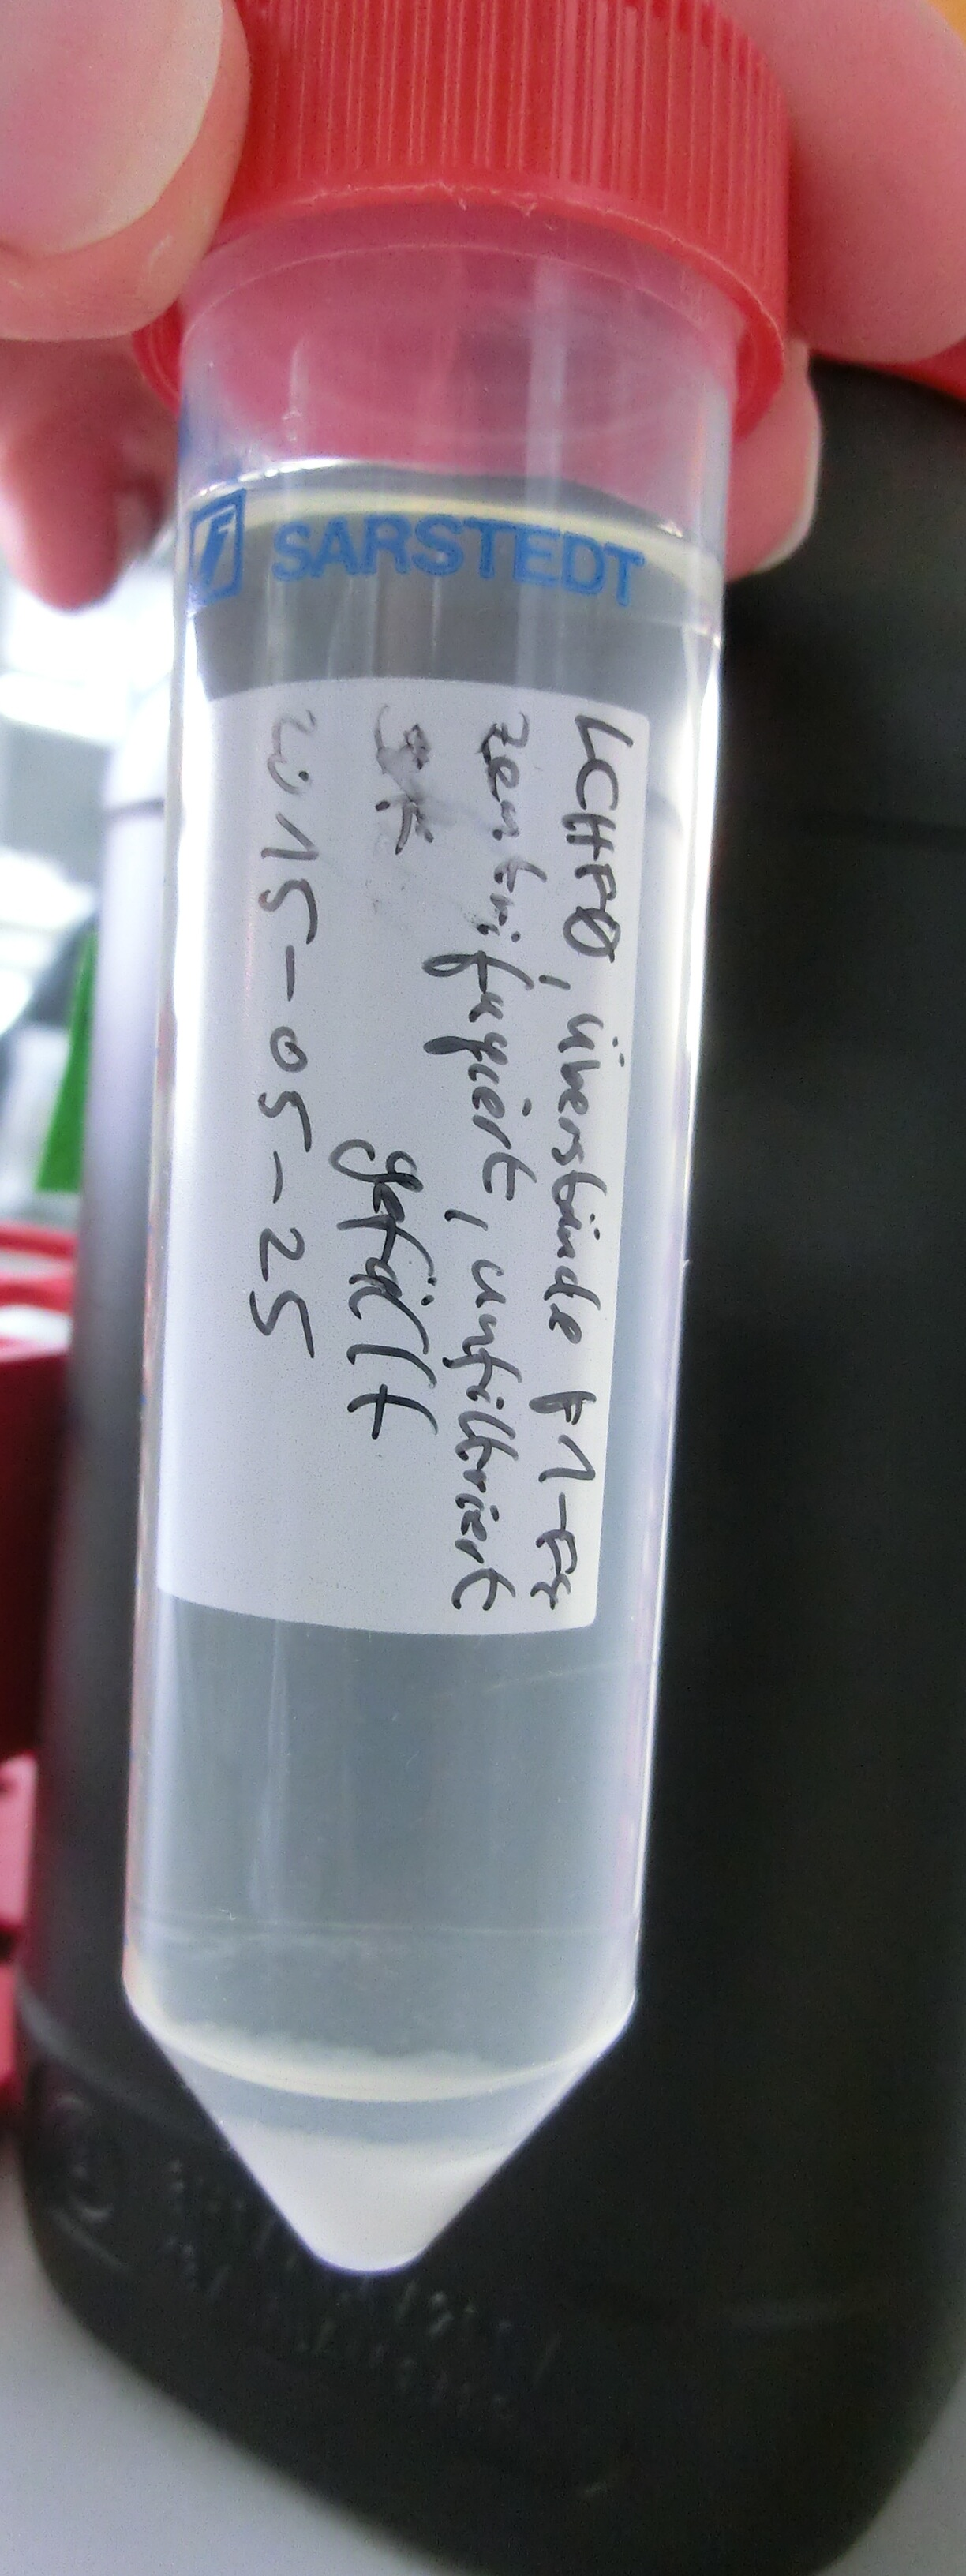
\includegraphics[height=180pt]{../doc/fig/lch-pf_block1_precipitate_before_CFF_presentation.jpg}}%
		\adjustbox{margin=0.15\textwidth{} 0ex}{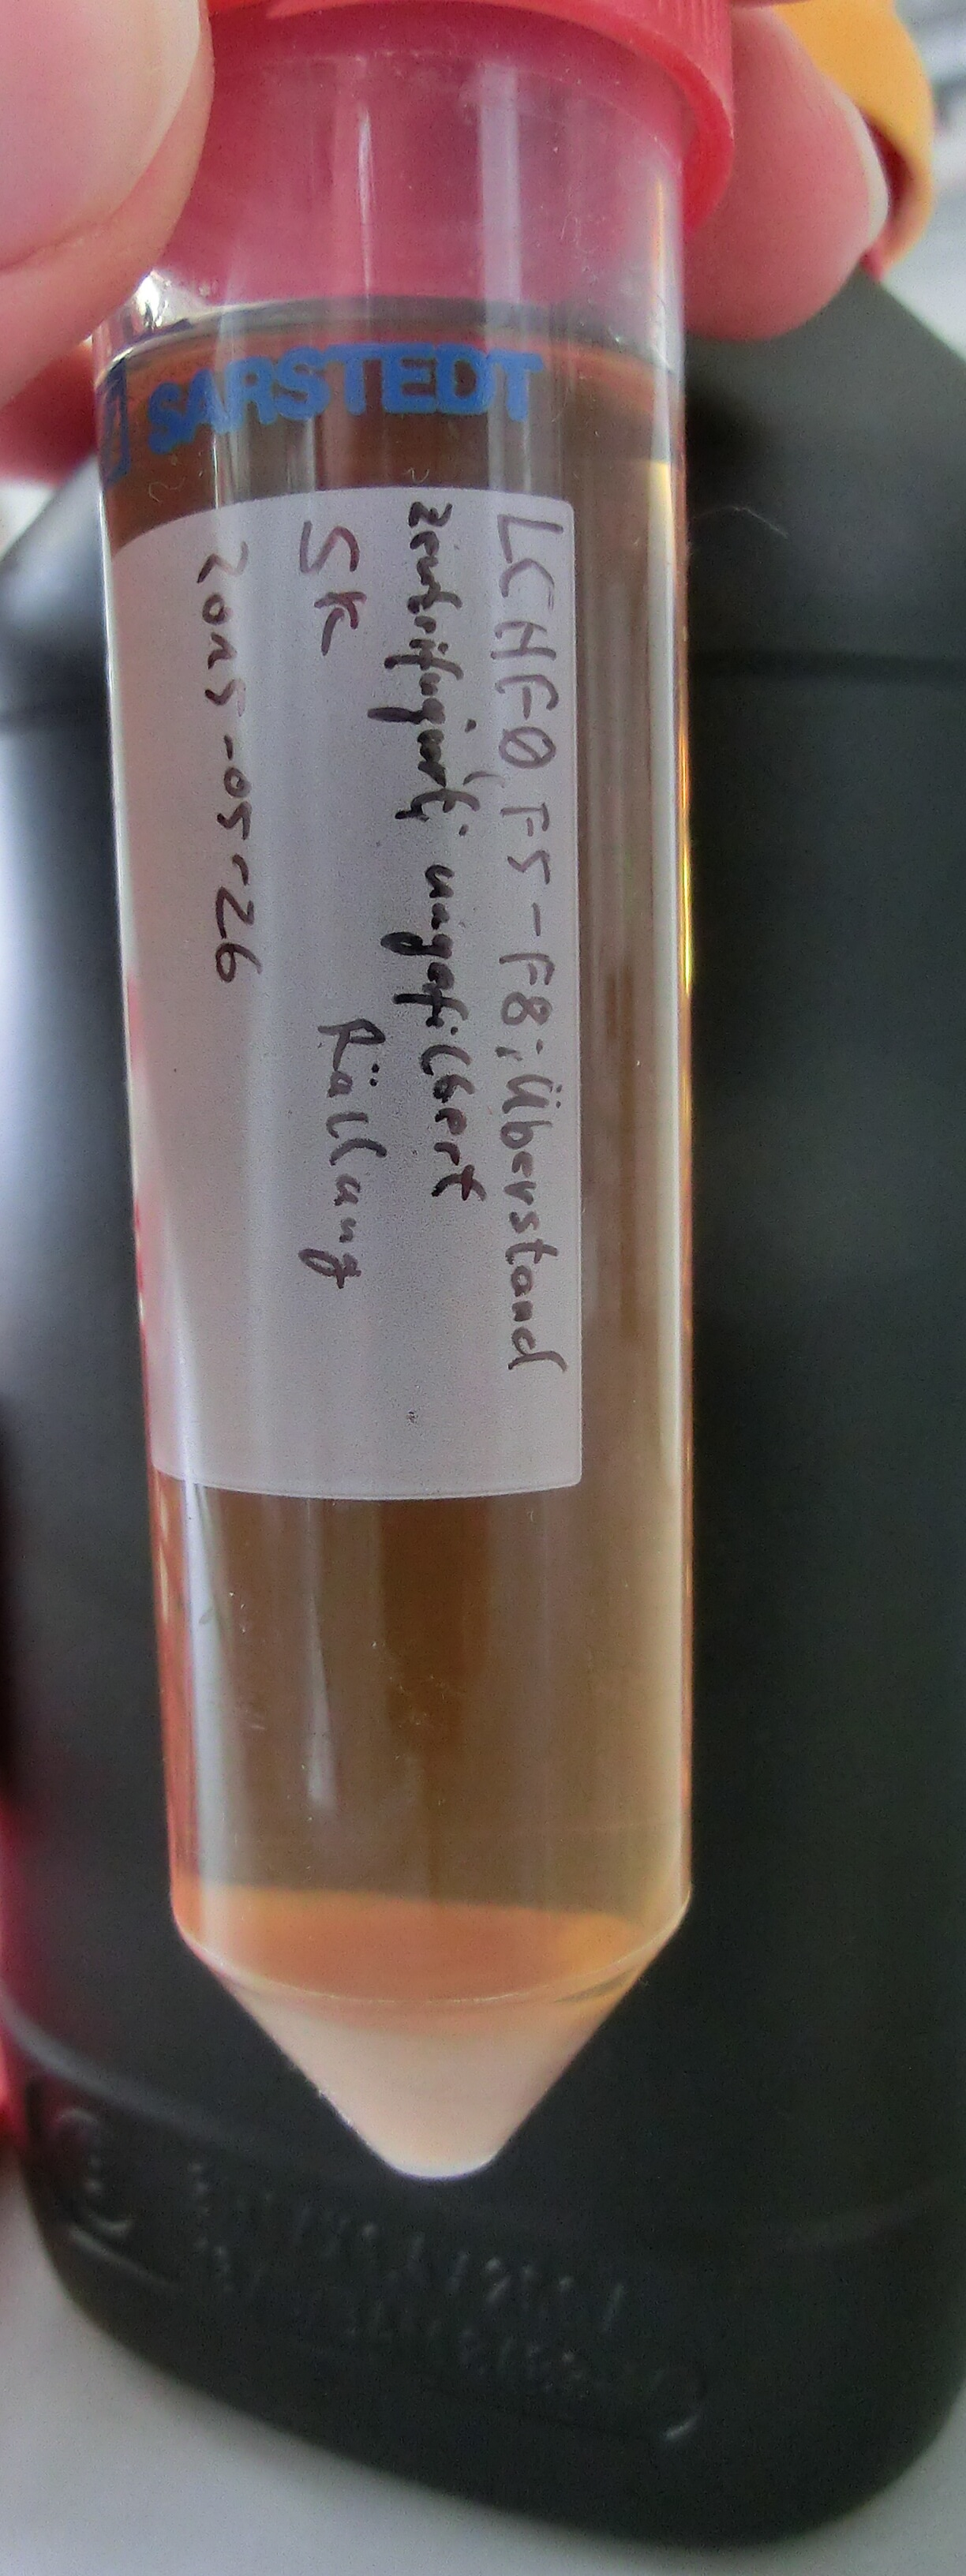
\includegraphics[height=180pt]{../doc/fig/lch-pf_block2_precipitate_before_CFF_presentation.jpg}}
	\end{center}
\end{frame}

\subsection{Outlook}

\begin{frame}{Outlook}{}
	\begin{itemize}
		\item Analytics: Monomer removal step before gel filtration
		\pause
		\item Optimization of screening steps
		\pause
		\item Pre-treatment of \lch{}
		\pause
		\item Optimization of the fermentation
		\pause
		\item Product purification
		\pause
			\begin{itemize}
				\item Cross-flow filtration with different solvents
				\pause
				\item Sugaring-out
			\end{itemize}
		\pause
		\item Strain engineering
		\pause
		\item Product characterization
	\end{itemize}
\end{frame}

\section{\SCL{} and \SHZ{} Production}

\begin{frame}{Introduction}{}
	\begin{itemize}
		\item Fungal \eps{}s \scl{} and \shz{}
		\pause
		\item Same? Similar?
		\pause
			\begin{itemize}
				\item Same, but ...
				\pause
				\item ... only selected fractions analysed
				\pause
				\item ... from our experience they \textit{are} different
			\end{itemize}
	\end{itemize}
\end{frame}

\begin{frame}{Fermentations}{\SCL{} from \rolf{} and \SHZ{} from \comm{}}
	\begin{itemize}
		\item Parallel fermentations with \rolf{} and \comm{}
		\item Analyses of \eps{}s (precipitates of supernatants)
		\pause
			\begin{itemize}
				\item Molar mass distribution
				\pause
				\item Dynamic viscosity
				\item Thixotropy
				\pause
				\item Solubility
				\pause
				\item Frequency of β-1,6-linked \glc{}
			\end{itemize}
		\pause
		\item Samples
			\begin{itemize}
				\item During the fermentations course
				\item At the end of the fermentation
			\end{itemize}
	\end{itemize}
\end{frame}

\begin{frame}{Results}{Cell Dry Masses}
	\begin{itemize}
		\item Cell dry masses increased with fermentation time
	\end{itemize}
	\begin{center}
		\includegraphics[width=0.6\textheight]{../doc/fig/fun-pf_cdm_600dpi.png}
	\end{center}
\end{frame}

\begin{frame}{Results}{Final \EPS{} Concentrations}
	\begin{itemize}
		\item \EPS{} concentrations tend to increase
		\item High value at \SIh{120}/low value at \SIh{144} of \comm{}
	\end{itemize}
	\begin{center}
		\includegraphics[width=0.6\textheight]{../doc/fig/fun-pf_eps-end_600dpi.png}
	\end{center}
\end{frame}

\begin{frame}{Results}{\EPS{} Courses}
	\begin{itemize}
		\item Drop after \SIh{24} caused by ten-fold dilution
	\end{itemize}
	\begin{center}
		\includegraphics[width=0.9\textwidth]{../doc/fig/fun-pf_eps-courses_600dpi.png}
	\end{center}
\end{frame}

\begin{frame}{Results}{\EPS{} Dissolution}
	\begin{itemize}
		\item \EPS{}s dissolved poorly
		\pause
		\item Solubility even low in DMSO
		\pause
			\begin{itemize}
				\item Something went \textit{very} wrong ...
				\pause
				\item All analyses rely on the solubility ...
			\end{itemize}
	\end{itemize}
\end{frame}

\subsection{Development of the Aniline Blue Assay}

\begin{frame}{Aniline Blue and Sirofluor}{Replacing Precipitation}
	\begin{itemize}
		\item Precipitation is cumbersome and error-prone
		\pause
		\item Wanted: Assay for direct determination
		\pause
		\item Found: Sirofluor, fluorescence dye
		\item Specificity: only glucans (β-1,3, β-1,3-β-1,6, α-1,4, α-1,4-α-1,6, cyclic α-1,4)
	\end{itemize}
	\pause
	\begin{center}
		\includegraphics[width=0.6\textwidth]{../doc/fig/Molecule_sirofluor_600dpi.png}
	\end{center}
	\pause
	\begin{itemize}
		\item No reasonable commercial source
		\pause
		\item But: Contamination of Aniline Blue
	\end{itemize}
\end{frame}

\begin{frame}{Aniline Blue and Sirofluor}{Fluorometric Quantification of β-1,3-β-1,6-Glucans \cite{Koenig2017}}
	\begin{itemize}
		\item Properties of the final assay
			\begin{itemize}
				\item Calibration range: \SImgpl{30} to \SIgpl{6} with $R^2 > \SIpct{99.8}$
				\pause
				\item Robustness
					\begin{itemize}
						\item \GLC{}: \SIgpl{50}
						\item Oxalic acid: \SIgpl{22.5}
						\item Potassium chloride: \SIgpl{13.3}
						\item Bovine serum albumine: \SIgpl{0.667}
					\end{itemize}
				\pause
				\item Reagent composition: \SImM{183} glycine, \SImM{229} \ce{NaOH}, \SImM{130} \ce{HCl}, \SImgpl{618} aniline blue in ultra-pure water. Final pH $\approx$ 9.9.
			\end{itemize}
		\pause
		\item Practical application
			\begin{itemize}
				\item Fermentation broth samples of \rolf{} and \comm{}
				\pause
				\item Comparison with precipitation, correction factors found
				\pause
					\begin{itemize}
						\item \rolf{}: 2.46 (supernatant after final centrifugation)
						\item \comm{}: 3.83 (blended broth)
					\end{itemize}
			\end{itemize}
	\end{itemize}
\end{frame}

\begin{frame}{Outlook}{}
	\begin{itemize}
		\item Precipitation optimization
		\pause
		\item Impurity reduction steps prior to precipitation
		\pause
		\item Improvements to the Aniline Blue assay
		\begin{itemize}
			\item More reliable than precipitation?
			\pause
			\item Sample pre-treatment to stabilize assay/supersede correction factors
		\end{itemize}
		\pause
		\item Adaptation/Development of other assays for quick qualitative overview of polymer types present
	\end{itemize}
\end{frame}

\begin{frame}{Thank you for your attention}{}

\end{frame}

\begin{frame}[allowframebreaks]{References}{}
	\printbibliography
\end{frame}

\end{document}
